\chapter{Gibbs Sampling in Prob. Submodular Models} \label{ch:gibbs}

\emph{The majority of the content of this chapter has already been published in conference proceedings \citep{gotovos15}.}

\section{Introduction}
In this chapter, we consider one of the simplest and most commonly used sampling procedures, namely the (single-site) Gibbs sampler, which is also known as the Glauber chain.
While there has been extensive work on the properties of the Gibbs sampler on low-order models, for example, Ising models \citep[Ch. 15]{levin08book}, not much is known about its behavior on higher-order models, except that, in general, we cannot hope for sub-exponential mixing times \citep{jerrum93}.
In fact, we show that even for probabilistic submodular models defined by monotone submodular functions, there are simple model families with exponential lower bounds on mixing time.

Our goal is to establish theoretical conditions that guarantee rapid mixing of the Gibbs sampler in probabilistic submodular models, and at the same time, investigate in what way the properties of sub- and supermodularity affect the resulting conditions.


\section{Problem Setup} \label{sect:setup}
In this chapter, we focus on distributions of the form
\begin{align}\label{eq:pdef}
p(S) = \frac{\exp(\beta F(S))}{Z},
\end{align}
for all $S \subseteq V$, where $F$ is submodular or supermodular.
We currently assume that $F$ is already learned or given, and omit the parameter vector $\btheta$ from the notation.
Furthermore, we have introduced a scaling parameter $\beta \geq 0$, which is referred to as inverse temperature, and will be useful for our subsequent theoretical analysis.
Intuitively, $\beta$ controls the concentration of $p$ around the high-value sets of $F$.
When $\beta = 0$, $p$ is the uniform distribution over $2^V$; when $\beta \to \infty$, the mass of $p$ fully concentrates around the maximizers of $F$.


\paragraph{Marginal inference.}
Our goal is to perform marginal inference for the distributions described above.
Concretely, for some fixed $A \subseteq B \subseteq V$, we would like to compute the probability of sets $S$ that contain all elements of $A$, but no elements outside of $B$, that is, $p(A \subseteq S \subseteq B)$.
More generally, we are interested in computing conditional probabilities of the form $p(A \subseteq S \subseteq B \mid C \subseteq S \subseteq D)$.
This computation can be reduced to computing unconditional marginals as follows.
For any $C \subseteq V$, define the contraction of $F$ on $C$, $F_C : 2^{V \setminus C} \to \mathbb{R}$, by $F_C(S) = F(S \cup C) - F(S)$, for all $S \subseteq V \setminus C$.
Also, for any $D \subseteq V$, define the restriction of $F$ to $D$, $F^D : 2^D \to \mathbb{R}$, by $F^D(S) = F(S)$, for all $S \subseteq D$.
If $F$ is submodular, then its contractions and restrictions are also submodular, and, thus, $(F_C)^D$ is submodular.
Finally, it is easy to see that $p(S \mid C \subseteq S \subseteq D) \propto \exp(\beta (F_C)^D(S))$.
In our experiments, we consider computing marginals of the form $p(i \in S \mid C \subseteq S \subseteq D)$, for some $i \in V$, which correspond to $A = \{i\}$, and $B = V$.

\paragraph{Submodular decomposition.}
In some of our following results we will use the fact that any submodular function $F$ can be written as
\begin{align} \label{eq:decomp}
  F = c + m + f,
\end{align}
where $c \in \mathbb{R}$ is a constant that has no effect on distributions defined by \eqref{eq:pdef}; $m$ is a normalized ($m(\varnothing) = 0$) modular function; and $f$ is a normalized ($f(\varnothing) = 0$) monotone submodular function, that is, it additionally satisfies the monotonicity property $f(i\mid S) \geq 0$, for all $i \in V$, and all $S \subseteq V$.
A similar decomposition is possible for any supermodular function as well.

\paragraph{The Gibbs sampler.}
We first set up some notation that is used throughout this chapter.
We denote by $\ss \defeq 2^V$ the state space, and by $P$ the transition matrix of the chain.
Each element $P(x, y)$ corresponds to the conditional probability of transitioning from state $x \in \ss$ to state $y \in \ss$, that is, $P(x, y) \defeq P(X_{t+1} = y \mid X_{t} = x)$, for any $x, y \in \ss$, and any $t \geq 0$.
We also define an adjacency relation $x \sim y$ on the elements of the state space, which denotes that $x$ and $y$ differ by exactly one element.
It follows that each $x \in \ss$ has exactly $n$ neighbors.

We define the Gibbs sampler by an iterative two-step procedure, as shown in \algoref{alg:gibbs}.
First, we select an element $i \in V$ uniformly at random; then, we add or removes $i$ to the current state $X_t$ according to the conditional probability of the resulting state.
In \figref{fig:gibbs} we illustrate one step of the Gibbs sampler on a small ground set $V = \{1, 2, 3\}$.
Assuming that the current state is $X_t = \{2\}$, there are three potential new next states, namely $\varnothing$, $\{1, 2\}$, or $\{2, 3\}$, which are the three neighbors of $X_t$ in the state space.
The Gibbs sampler first selects one of the neighbors uniformly at random, and then either stays at $X_t$ or moves to that neighbor according to the corresponding conditional probability.

%\RestyleAlgo{ruled,vlined,linesnumbered}
\begin{algorithm}[tb]
    \setstretch{1.3}
    \DontPrintSemicolon
    \vspace{0.5em}
    \SetKwInOut{Input}{Input}
    \Input{Ground set $V$, distribution $p(S) \propto \exp(\beta F(S))$}
	$X_0$ $\gets$ random subset of $V$\\
	\For{$t = 0$ \KwTo $N_{\mathrm{iter}}$}{
	  $i$ $\gets$ $\mathrm{Unif}(V)$\;
	  $\Delta_F(i \mid X_t)$ $\gets$ $F(X_t \cup \{i\}) - F(X_t \setminus \{i\})$\;
	  $p_{\mathrm{add}}$ $\gets$ $\exp(\beta\Delta_F(i \mid X_t))/(1 + \exp(\beta\Delta_F(i \mid X_t)))$\;
	  $z$ $\gets$ $\mathrm{Unif}([0,1])$\;
	  \uIf{$z \leq p_{\mathrm{add}}$}{
        $X_{t+1} \gets X_t \cup \{i\}$\;
      } \Else{
        $X_{t+1} \gets X_t \setminus \{i\}$\;
      }}
    %\vspace{1em}
	\caption{The Gibbs sampler for probabilistic submodular models.}
	\label{alg:gibbs}
\end{algorithm}

\begin{figure}[htb]
\centering
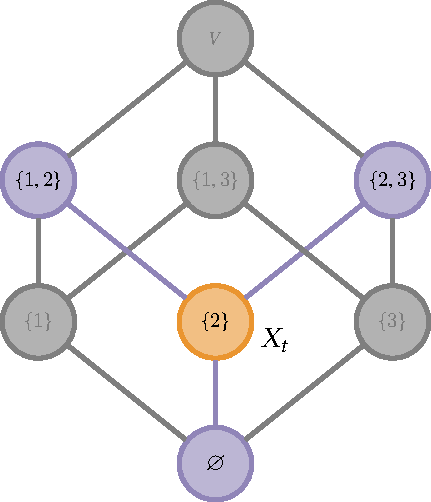
\includegraphics[width=0.55\textwidth]{figures/gibbs/lattice_gibbs_2.pdf}\\[1em]
\caption{An illustration of a single Gibbs step on ground set $V = \{1, 2, 3\}$, and current state $X_t = \{2\}$.
We first choose one of the neighbors of $X_t$ uniformly at random, and then either stay at $X_t$ or move to that neighbor according to the corresponding conditional probability.}
\label{fig:gibbs}
\end{figure}

The important thing to note here is that the computed conditional probabilities do not depend on the partition function $Z$, thus the chain can be simulated efficiently, even though $Z$ is unknown and hard to compute.
Moreover, it is easy to see that
\begin{align*}
\Delta_F(i \mid X_t) = \llbracket i\not\in X_t\rrbracket F(i \mid X_t) + \llbracket i\in X_t\rrbracket F(i \mid X_t\setminus\{i\}).
\end{align*}
Therefore, the sampler only requires a black box for the marginal gains of $F$, which are often faster to compute in practice than the values of $F$ itself.
Finally, it is easy to show that the stationary distribution of the chain constructed this way is $p$.

\section{Hardness of Inference}
Performing exact inference in probabilistic submodular models is, in general, computationally infeasible.
Only for very few exceptions, such as determinantal point processes, is exact inference possible in polynomial time \citep{kulesza12}.
As we mentioned before, even approximating the partition function of general Ising models---a subclass of PSMs---is a hard problem; in particular, there is no FPRAS for this problem, unless RP = NP \citep{jerrum93}.
This implies that the mixing time of any Markov chain with such a stationary distribution will, in general, be exponential in $n$.

\subsection{Example: Log-submodular Grid}
To further highlight the hardness of inference in the general models we consider, we show that even for distributions defined through a seemingly benign subclass of submodular functions, mixing times can be exponential in $n$.
We say that a set function $F : 2^V \to \mathbb{R}$ is monotone, if $F(i \mid S) \geq 0$, for all $i \in V$, and all $S \subseteq V$.
Intuitively, adding elements to our set always leads to higher values.

\todo{Introduce Metropolis either here or in the background chapter.}
For the purposes of the following proposition, we will use a Metropolis chain, rather than a Gibbs chain, to simplify the exposition.
While the two chains are not identical, they share the same principle of making local moves by considering ratios of probabilities of neighboring states.
\begin{prop}
There is a family of monotone submodular functions $(F_n)_n$, such that, for the corresponding log-submodular family of distributions $(p_n)_n$ defined as in \eqref{eq:pdef}, the Metropolis chain has mixing time
\begin{align*}
  \tm  = \Omega(2^{n/2}),
\end{align*}
for any value of $\beta$.
\end{prop}

\begin{proof}
The functions used to prove the above lemma are based on the following construction.
For any even $n \geq 2$, let $V_n = \{1,\ldots,n\}$, $R_n = \{1,\ldots,n/2\}$, and $C_n = \{n/2+1,\ldots,n\}$.
To define function $F_n : 2^{V_n} \to \mathbb{R}$, we conceptually use a $n/2 \times n/2$ square grid, whose rows are indexed by $R$ and columns by $C$.
Each cell $(i, j)$ of the grid is considered to be covered, if either row $i \in R$ or column $j \in C$ is selected.
Formally, we define $F_n$ by
\begin{align*}
  F_n(S) = \frac{4}{n^2}\big\vert \sdef{(i, j) \in R \times C}{i \in S \lor j \in S}\big\vert,
\end{align*}
for any $S \subseteq V_n$, which results in $F_n(V_n) = 1$.
\figref{fig:submod_grid} shows an example of such a grid construction.

\begin{figure}[htb]
  \centering
  \begin{tikzpicture}[
	%baseline,
	scale=0.9
	]
    
	\fill[col1] (0,3) rectangle (4,4);
	\fill[col1] (0,1) rectangle (4,2);
	\fill[col1] (2,0) rectangle (3,4);
	\draw[step=1cm,black!70!white,line width=1.5pt] (0,0) grid (4,4);
	
	\node at (-0.3,3.5) {\sffamily 1};
	\node at (-0.3,2.5) {\sffamily 2};
	\node at (-0.3,1.5) {\sffamily 3};
	\node at (-0.3,0.5) {\sffamily 4};
	\node at (0.5,4.3) {\sffamily 5};
	\node at (1.5,4.3) {\sffamily 6};
	\node at (2.5,4.3) {\sffamily 7};
	\node at (3.5,4.3) {\sffamily 8};
\end{tikzpicture}\\[1em]
  \caption{Example grid for $n = 8$ with the cells corresponding to $F_8(\{1,3,7\}) = 10/16$ shown shaded.}
  \label{fig:submod_grid}
\end{figure}

\newcommand{\hrn}{\mathcal{R}_n}
\newcommand{\hcn}{\mathcal{C}_n}
\newcommand{\hkn}{\mathcal{K}_n}
\newcommand{\htn}{\mathcal{T}_n}

Furthermore, if we define $\hrn = \{S \subseteq V \mid R \subseteq S\}$, $\hcn = \{S \mid C \subseteq S \subseteq V\}$, and $\hkn = 2^V \setminus (\hrn \cup \hcn)$, then the following properties hold.
\begin{align}
  &|\hrn| = |\hcn| = 2^{n/2} \label{eq:prop1} \\
  &\hrn \cap \hcn = \{V\} \label{eq:prop2} \\
  &\forall S \in \hrn\cup\hcn,\ f(S) = 1 \label{eq:prop3} \\
  &\forall S \in \hkn,\ f(S) \leq 1 - 4/n^2 \label{eq:prop4}.
\end{align}
Assume a Metropolis chain with transition matrix $P$, and stationary distribution $p_n(S) \propto \exp(\beta F_n(S))$.
To prove a lower bound on the mixing time of this chain, we are going to upper bound the bottleneck ratio \citep[Ch. 7]{levin08} of set $\htn = \hrn \setminus \{V\}$, defined as
\begin{align*}
  \Phi(\htn) = \frac{Q(\htn, \htn^c)}{\pi(\htn)} = \frac{Q(\htn, \hcn) + Q(\htn, \hkn)}{\pi(\htn)},
\end{align*}
where $\htn^c = 2^V \setminus \htn$ is the complement of $\htn$. We now compute or bound each of the terms $\pi(\htn)$, $Q(\htn, \hcn)$, and $Q(\htn, \hkn)$.

\paragraph{Computing $\pi(\htn)$.}
\begin{align*}
  \pi(\htn) &= |\htn| \frac{e^{\beta}}{Z} \tag*{by \eqref{eq:prop3}} \\
         &= (2^{n/2} - 1) \frac{e^{\beta}}{Z}. \tag*{by \eqref{eq:prop1}}
\end{align*}
Note that, by an analogous derivation, we get $\pi(\hcn \setminus \{V\}) = \pi(\htn)$ and, by \eqref{eq:prop2},
\begin{align*}
  &\pi(\htn) + \pi(\hcn \setminus \{V\}) < 1 \\
  \Rightarrow\ \ &\pi(\htn) < 0.5.
\end{align*}
  
\paragraph{Computing $Q(\htn, \hcn)$.}
\begin{align*}
  Q(\htn, \hcn) &= \sum_{x \in \htn} Q(x, \hcn) \\
                &= \sum_{x \in \htn} Q(x, \{V\}) \tag*{by \eqref{eq:prop2}} \\
                &= \sum_{x \in \htn} \frac{1}{2n} \frac{e^{\beta}}{Z} \tag*{by \eqref{eq:prop3}} \\
                &= n \frac{1}{2n} \frac{e^{\beta}}{Z} = \frac{e^{\beta}}{2Z}.
\end{align*}
    
\paragraph{Bounding $Q(\htn, \hkn)$.}
\begin{align*}
  Q(\htn, \hkn) &= \sum_{x \in \htn} Q(x, \hkn) \\
                &\leq \sum_{x \in \htn} \frac{1}{2n} \frac{e^{\beta - 4\beta/n^2}}{Z} \tag*{by \eqref{eq:prop4}} \\
                &= \frac{2^{n/2} - 1}{2n} \frac{e^{\beta - 4\beta/n^2}}{Z}. \tag*{by \eqref{eq:prop1}}
\end{align*}

\paragraph{Bounding $\Phi(\htn)$.}
\begin{align*}
  \Phi(\htn) &\leq \frac{1}{2^{n/2} - 1}\left(\frac{1}{2} + \frac{(2^{n/2} - 1) e^{-4\beta/n^2}}{2n}\right)\\
          &= \frac{1}{2(2^{n/2} - 1)} + \frac{e^{-4\beta/n^2}}{2n}.
\end{align*}
Using Theorem 7.3 \citep{levin08book}, it follows that
\begin{align*}
  \tm(1/4) \geq \frac{1}{4\Phi(\htn)} = \Omega(2^{n/2}).
\end{align*}

\end{proof}

\section{Polynomial-time mixing} \label{sect:poly}
Our first result provides conditions that guarantee polynomial mixing times in the size of the ground set $n$.
As we will see, the conditions depend crucially on the following quantity, which is defined for any set function $F : 2^V \to \mathbb{R}$:
\begin{align*}
  \zf \defeq \max_{A, B \subseteq V} \left|F(A) + F(B) - F(A \cup B) - F(A \cap B) \right|.
\end{align*}
Intuitively, $\zf$ quantifies a notion of distance to modularity.
To see this, note that a function $F$ is modular if and only if $F(A) + F(B) = F(A \cup B) + F(A \cap B)$, for all $A, B \subseteq V$.
For modular functions, therefore, we have $\zf = 0$.
Furthermore, a function $F$ is submodular if and only if $F(A) + F(B) \geq F(A \cup B) + F(A \cap B)$, for all $A, B \subseteq V$.
Similarly, $F$ is supermodular if the above holds with the sign reversed.
It follows that for submodular and supermodular functions, $\zf$ represents the worst-case amount by which $F$ violates the modular equality.
It is also important to note that, for submodular and supermodular functions, $\zf$ depends only on the monotone part of $F$; if we decompose $F$ according to \eqref{eq:decomp}, then it is easy to see that $\zf = \zeta_f$.
A trivial upper bound on $\zf$, therefore, is $\zf \leq f(V)$.
Another quantity that has been used in the past to quantify the deviation of a submodular function from modularity is the curvature \cite{conforti84}, defined as $\kappa_F \defeq 1 - \min_{i \in V} \left(F(i\mid V\setminus\{i\}) / F(i)\right)$.
Although of similar intuitive meaning, the multiplicative nature of its definition makes it significantly different from $\zf$, which is defined additively.

\paragraph{Examples.}
As an example of a function class with $\zf$ that do not depend on $n$, assume a ground set $V = \bigcup_{\ell = 1}^L V_{\ell}$, and consider functions of the form
\begin{align*}
F(S) = \sum_{\ell = 1}^L \phi(|S \cap V_{\ell}|),
\end{align*}
where $\phi : \mathbb{R} \to \mathbb{R}$ is a bounded concave function, for example, $\phi(x) = \min\{\phi_{\max}, x\}$.
Functions of this form are submodular, and have been used in applications such as document summarization to encourage diversity \citep{lin11}.
It is easy to see that, for such functions, $\zf \leq L\phi_{\max}$, that is, $\zf$ is independent of $n$.

For the \flid{} model \todo{ref}, we have $f(S) = \sum_{j=1}^L \max_{i \in S} w_{ij}$, therefore we get $\zf \leq f(V) = \sum_{j=1}^L w_j^{\mathrm{max}}$, where $w_j^{\mathrm{max}} = \max_{i \in V} w_{ij}$.
Since the values of $\bw$ depend primarily on the number of repulsive groups, rather than the size of the ground set, we expect $\zf$ to grow much slower than $n$ in most practical applications.

\vspace{1.5em}
\noindent The following theorem establishes a bound on the mixing time of the Gibbs sampler run on models of the form \eqref{eq:pdef}.
The bound is exponential in $\zf$, but polynomial in $n$.
\begin{theorem} \label{thm:poly}
  For any function $F : 2^V \to \mathbb{R}$, the mixing time of the Gibbs sampler is bounded by
  \begin{align*}
    \tme \leq 2n^2 \exp(2 \beta \zf) \log\left(\frac{1}{\epsilon p_{\min}}\right),
  \end{align*}
  where $p_{\min} \defeq \displaystyle\min_{S \in \ss}p(S)$.
  If $F$ is submodular or supermodular, then the bound is improved to
  \begin{align*}
    \tme \leq 2n^2 \exp(\beta \zeta_f) \log\left(\frac{1}{\epsilon p_{\min}}\right).
  \end{align*}
\end{theorem}
Note that, since the factor of two that constitutes the difference between the two statements of the theorem lies in the exponent, it can have a significant impact on the above bounds.
The dependence on $p_{\min}$ is related to the (worst-case) starting state of the chain, and can be eliminated if we have a way to guarantee a high-probability starting state.
If $F$ is submodular or supermodular, this is usually straightforward to accomplish by using one of the standard constant-factor optimization algorithms \citep{nemhauser78,fujishige05} as a preliminary step.
More generally, if $F$ is bounded by $0 \leq F(S) \leq F_{\max}$, for all $S \subseteq V$, then $\log (1/p_{\min}) = \mathcal{O}(n \beta F_{\max})$.

\paragraph{Canonical paths}
Our proof of \theoremref{thm:poly} is based on the method of \emph{canonical paths} \citep{jerrum03,sinclair92,jerrum89,diaconis91}.
The high-level idea of this method is to view the state space as a graph, and try to construct a path between each pair of states, which carries a certain amount of flow specified by the stationary distribution under consideration.
Depending on the choice of these paths and the resulting load on the edges of the graph we can derive bounds on the mixing time of the Markov chain.

More concretely, let us assume that for some set function $F$ and corresponding distribution $p$ as in \eqref{eq:pdef}, we construct the Gibbs chain on state space $\ss = 2^V$ with transition matrix $P$.
We can view the state space as a directed graph that has vertex set $\ss$, and for any $A, B \in \ss$, contains edge $(S, S')$ if and only if $S \sim S'$, that is, if and only if $S$ and $S'$ differ by exactly one element.
Now, for any pair of states $A, B \in \ss$, we define a \emph{canonical path}
\begin{align*}
\gamma_{AB} \defeq (A = S_0, S_1, \ldots, S_{\ell} = B),
\end{align*}
such that all $(S_i, S_{i+1})$ are edges in the above graph.
We denote the length of path $\gamma_{AB}$ by $|\gamma_{AB}|$, and define $Q(S, S') \defeq p(S) P(S, S')$.
We also denote the set of all pairs of states whose canonical path goes through $(S, S')$ by
\begin{align*}
\mathcal{C}_{SS'} \defeq \sdef{(A, B) \in \ss \times \ss}{(S, S') \in \gamma_{AB}}.
\end{align*}
The following quantity, referred to as the \emph{congestion} of an edge, uses a collection of canonical paths to quantify to what amount that edge is overloaded:
\begin{align} \label{eq:cong}
  \rho(S, S') \defeq \frac{1}{Q(S, S')} \sum_{(A, B) \in \mathcal{C}_{SS'}} p(A) p(B) |\gamma_{AB}|.
\end{align}
The denominator $Q(S, S')$ quantifies the capacity of edge $(S, S')$, while the sum represents the total flow through that edge according to the choice of canonical paths.
The congestion of the whole graph is then defined as $\rho \defeq \max_{S \sim S'}\rho(S, S')$.
Low congestion implies that there are no bottlenecks in the state space, and the chain can move around fast, which results in rapid mixing.
The following theorem makes this statement more concrete.

\begin{theorem}[\hspace{1sp}\citealp{sinclair92,jerrum03}] \label{thm:cpath}
  For any collection of canonical paths with congestion $\rho$, the mixing time of the chain is bounded by
  \begin{align*}
  	\tme \leq \rho \log\left(\frac{1}{\epsilon p_{\mathrm{min}}}\right).
  \end{align*}
%  where $p_{\min} \defeq \displaystyle\min_{S \in \ss}p(S)$.
\end{theorem}

\subsection{Proof of \theoremref{thm:poly}}
To apply \theoremref{thm:cpath} to our class of distributions, we need to construct a set of canonical paths in the corresponding state space $2^V$, and upper bound the resulting congestion.
First, note that, to transition from state $A \in \ss$ to state $B \in \ss$, in our case, it is enough to remove the elements of $A \setminus B$ and add the elements of $B \setminus A$.
Each removal and addition corresponds to an edge in the state space graph, and the order of these operations identify a canonical path in this graph that connects $A$ to $B$.
For our analysis, we assume a fixed order on $V$ (e.g., the natural order of the elements themselves), and perform the operations according to this order.

Having defined the set of canonical paths, we proceed to bounding the congestion $\rho(S, S')$ for any edge $(S, S')$.
The main difficulty in bounding $\rho(S, S')$ is due to the sum in \eqref{eq:cong} over all pairs in $\mathcal{C}_{SS'}$.
To simplify this sum, we construct for each edge $(S, S')$ an injective map $\ess : \mathcal{C}_{SS'} \to \ss$; this is a combinatorial encoding technique that has been previously used in similar proofs to ours \citep{jerrum03}.
The following lemma details this construction, where for sets $A, B$, we denote $A \oplus B \defeq (A \setminus B)\cup(B \setminus A)$.

\begin{lemma} \label{lem:inj}
Define the maps $\ess : \mathcal{C}_{SS'} \to \ss$, for each pair $(S, S') \in \ss \times \ss$ with $S \sim S'$, as follows:
\begin{align*}
  \ess(A, B) = \twopartdefo{A \oplus B \oplus S}{F(S') \geq F(S)}{A \oplus B \oplus S'}.
\end{align*}
Then, each map $\ess$ is injective.
\end{lemma}

\begin{proof}
  Assume that $F(S') \geq F(S)$, and $S' = S \cup \{r\}$, for some $r \in V$.
  Assume that we are given $C \defeq A \oplus B \oplus S$, and we want to recover $A$ and $B$.
  We will denote by $\prec$ the natural ordering of the ground set $V$.
  First, we define
  \begin{align*}
    K^- &\defeq \sdef{i \in C \oplus S}{i \prec r}\\
    K^+ &\defeq \sdef{i \in C \oplus S}{i \succ r}.
  \end{align*}
  Then, we can recover $A$ and $V$ as follows:
  \begin{align*}
    A &= S \oplus K^-\\
    B &= S' \oplus K^+.
  \end{align*}
  The case $S' = S \setminus \{r\}$, as well as the two cases for $F(S') < F(S)$ are completely analogous.
  Note that the distinction based on the value of the function has no effect on the proof here, but is technically needed for the next lemma.
  The only thing that changes between the cases is whether the element $r$ that gets added or removed in the transition $(S, S')$ belongs to $A$ or $B$, which is always straightforward to determine from the type of the transition (for additions it belongs to $B$, and for removals to $A$).
\end{proof}
\noindent We then prove the following key lemma about the maps constructed above.
\begin{lemma} \label{lem:poly_full}
  For any $S \sim S'$, and any $A, B \in \ss$, it holds that
  \begin{align*}
    p(A)p(B) \leq 2n\exp(2 \beta \zf)Q(S, S')p(\ess(A, B)).
  \end{align*}
  
  If $F$ is submodular or supermodular, then the bound is improved to
  \begin{align*}
  	p(A)p(B) \leq 2n\exp(\beta \zeta_f)Q(S, S')p(\ess(A, B)).
  \end{align*}
\end{lemma}
\begin{proof}
  We will consider the case $S' = S \cup \{r\}$, for some $r \in V$, with $F(S') \geq F(S)$.
  Again, the other three cases are completely analogous by using $\ess$ as defined in \lemmaref{lem:inj}.
  
  We first compute
  \begin{align*}
    Q(S, S') &= p(S)P(S, S')\\
             &= \frac{1}{n}\frac{p(S)p(S')}{p(S) + p(S')} \tag*{by definition of the Gibbs sampler}\\
             &= \frac{1}{nZ}\frac{\exp(\beta F(S)) \exp(\beta F(S'))}{\exp(\beta F(S)) + \exp(\beta F(S'))} \tag*{by definition of our models}\\
             &\geq \frac{1}{nZ}\frac{\exp(\beta F(S)) \exp(\beta F(S'))}{2\exp(\beta F(S'))} \tag*{by $F(S') \geq F(S)$}\\
             &= \frac{\exp(\beta F(S))}{2nZ}.
  \end{align*}
  As a result, we get
  \begin{align} \label{eq:ppq}
    \frac{p(A)p(B)}{Q(S, S')} \leq \frac{2n}{Z}\exp(\beta (F(A) + F(B) - F(S))).
  \end{align}
  Let us denote
  \begin{align*}
    \zf(A, B) \defeq F(A) + F(B) - F(A \cup B) - F(A \cap B),
  \end{align*}
  for any $A, B \subseteq V$, so that $\zf = \max_{A, B \subseteq V}|\zf(A, B)|$.
  Then, if we denote
  \begin{align*}
    C \defeq \ess(A, B) = A \oplus B \oplus S,
  \end{align*}
  we have
  \begin{align*}
    &F(A) + F(B) - F(S)\\
    &= (F(A) + F(B) - F(A \cup B) - F(A \cap B)) -\\
    &\ \ \ \ \ (F(S) + F(C) - F(A \cup B) - F(A \cap B)) + F(C)\\
    &= (F(A) + F(B) - F(A \cup B) - F(A \cap B)) -\\
    &\ \ \ \ \ (F(S) + F(C) - F(S \cup C) - F(S \cap C)) + F(C)\\
    &= \zf(A, B) - \zf(S, C) + F(C)\\
    &\leq 2\zf + F(C).
  \end{align*}
  If $F$ is submodular, then $\zf(A, B)$ and $\zf(S, C)$ are both non-negative, therefore $\zf(A, B) - \zf(S, C) + F(C) \leq \zf + F(C) = \zeta_f + F(C)$.
  Similarly, if $F$ is supermodular, then $\zf(A, B)$ and $\zf(S, C)$ are both non-positive, therefore $\zf(A, B) - \zf(S, C) + F(C) \leq \zf + F(C) = \zeta_f + F(C)$.
  Substituting these bounds in \eqref{eq:ppq} gives us the result of the lemma.
\end{proof}
Since $\ess$ is injective, it follows that $\sum_{(A, B) \in \mathcal{C}_{SS'}} p(\ess(A, B)) \leq 1$.
Furthermore, it is clear that each canonical path $\gamma_{AB}$ has length $|\gamma_{AB}| \leq n$, since we need to add and/or remove at most $n$ elements to get from state $A$ to state $B$.
Combining these two facts with the above lemma, we get
\begin{align*}
  \rho(S, S') \leq 2n^2 \exp(2 \beta \zf),
\end{align*}
for any set function $F$, and
\begin{align*}
  \rho(S, S') \leq 2n^2 \exp(2 \beta \zeta_f),
\end{align*}
if $F$ is sub- or supermodular.


\section{Fast mixing}
We now proceed to show that, under some stronger conditions, we are able to establish even faster---$\mathcal{O}(n \log n)$---mixing.
For any function $F$, we denote
\begin{align*}
\D_F(i\mid S) \defeq F(S \cup \{i\}) - F(S \setminus \{i\}),
\end{align*}
and define the following quantity,
\begin{align*}
  \gf &\defeq \max_{\substack{S \subseteq V\\r \in V}} \sum_{\substack{i \in V}} \tanh\left(\frac{\beta}{2} \Big|\D_F(i\mid S) - \D_F(i\mid S \cup \{r\})\Big| \right),
\end{align*}
which quantifies the (maximum) total influence of an element $r \in V$ on the values of $F$.
For example, if the inclusion of $r$ makes no difference with respect to other elements of the ground set, we will have $\gf = 0$.
The following theorem establishes conditions for fast mixing of the Gibbs sampler when run on models of the form \eqref{eq:pdef}.

\begin{theorem} \label{thm:fast}
  For any set function $F : 2^V \to \mathbb{R}$, if $\gf < 1$, then the mixing time of the Gibbs sampler is bounded by
  \begin{align*}
  	\tme \leq \frac{1}{1 - \gf}n(\log n + \log \frac{1}{\epsilon}).
  \end{align*}
  If $F$ is additionally submodular or supermodular, and is decomposed according to \eqref{eq:decomp}, then
  \begin{align*}
  	\tme \leq \frac{1}{1 - \gsf}n(\log n + \log \frac{1}{\epsilon}).
  \end{align*}
\end{theorem}
Note that, in the second part of the theorem, $\gsf$ depends only on the monotone part of $F$. 

\paragraph{Coupling.}
Our proof of \theoremref{thm:fast} is based on the \emph{coupling} technique \citep{aldous83}; more specifically, we use the \emph{path coupling} method \citep{bubley97,levin08,jerrum03}.
Given a Markov chain $(Z_t)$ on state space $\ss$ with transition matrix $P$, a coupling for $(Z_t)$ is a new Markov chain $(X_t, Y_t)$ on state space $\ss \times \ss$, such that both $(X_t)$ and $(Y_t)$ are by themselves Markov chains with transition matrix $P$.
The idea is to construct the coupling in such a way that, even when the starting points $X_0$ and $Y_0$ are different, the chains $(X_t)$ and $(Y_t)$ tend to coalesce.
Then, it can be shown that the coupling time $t_{\mathrm{couple}} \defeq \min\sdef{t \geq 0}{X_t = Y_t}$ is closely related to the mixing time of the original chain $(Z_t)$ \citep{levin08}.

The main difficulty in applying the coupling approach lies in the construction of the coupling itself, for which one needs to consider any possible pair of states $(X_t, Y_t)$.
The path coupling technique makes this construction easier by utilizing the same state-space graph that we used to define canonical paths in \sectref{sect:poly}.
The core idea is to first define a coupling only over adjacent states, and then extend it for any pair of states by using a metric on the graph.
More concretely, let us denote by $d : \ss \times \ss \to \mathbb{R}$ the \emph{path metric} on state space $\ss$; that is, for any $x, y \in \ss$, $d(x, y)$ is the minimum length of any path from $x$ to $y$ in the state space graph.
The following theorem establishes fast mixing using this metric, as well as the diameter of the state space, $\mathrm{diam}(\ss) \defeq \max_{x,y \in \ss}d(x, y)$.
\begin{theorem}[\hspace{1sp}\citealp{bubley97,levin08}] \label{thm:pc}
For any Markov chain $(Z_t)$, let $(X_t, Y_t)$ be a coupling, such that, for some $a \geq 0$, and any $x, y \in \ss$ with $x \sim y$, it holds that
\begin{align*}
  \E[d(X_{t+1}, Y_{t+1}) \mid X_t = x, Y_t = y] \leq e^{-\alpha}d(x, y).
\end{align*}
Then, the mixing time of the original chain $(Z_t)$ is bounded by
\begin{align*}
  \tme \leq \frac{1}{\alpha}\left(\log(\mathrm{diam}(\ss)) + \log\frac{1}{\epsilon} \right).
\end{align*}
\end{theorem}

\subsection{Proof of \theoremref{thm:fast}}
In our case, the path metric $d$ is the Hamming distance between the binary vectors representing the states (equivalently, the number of elements by which two sets differ).
We need to construct a suitable coupling $(X_t, Y_t)$ for any pair of states $x \sim y$.
Consider the two corresponding sets $S, R \subseteq V$ that differ by exactly one element, and assume that $R = S \cup \{r\}$, for some $r \in V$. (The case $S = R \cup \{s\}$ for some $s \in V$ is completely analogous.)
Remember that the Gibbs sampler first chooses an element $i \in V$ uniformly at random, and then adds or removes it according to the conditional probabilities.
Our goal is to make the same updates happen to both $S$ and $R$ as frequently as possible.
As a first step, we couple the candidate element for update $i \in V$ to always be the same in both chains.
Then, we have to distinguish between the following cases.

If $i = r$, then the conditionals for both chains are identical, and we can couple both chains to add $r$ with probability
\begin{align*}
p_{\mathrm{add}} \defeq \frac{p(S \cup \{r\})}{p(S) + p(S \cup \{r\})},
\end{align*}
which will result in new sets $S' = R' = S \cup \{r\}$, or remove $r$ with probability $1 - p_{\mathrm{add}}$, which will result in new sets $S' = R' = S$.
Either way, we will have $d(S', R') = 0$.
  
If $i \neq r$, we cannot always couple the updates of the chains, because the conditional probabilities of the updates are different.
In fact, we are forced to have different updates---one chain adding $i$, the other chain removing $i$---with probability equal to the difference of the corresponding conditionals, which we denote here by $p_{\mathrm{dif}}(v)$, defined as follows,
\begin{align*}
  p_{\mathrm{dif}}(i) \defeq \left|\frac{p(S \cup \{i\})}{p(S \cup \{i\}) + p(S \setminus \{i\})} - \frac{p(R \cup \{i\})}{p(R \cup \{i\}) + p(R \setminus \{i\})}\right|.
\end{align*}
In the case of different updates, we have $d(S', R') = 2$, otherwise the chains make the same update and still differ only by element $r$, that is, $d(S', R') = 1$.

Putting together the three possible cases for the value of $d(S', R')$ described above, we get the following expected distance after one step,
\begin{align*}
  \E[d(S', R')] = 1 -\frac{1}{n} + \frac{1}{n}\sum_{i \neq r}p_{\mathrm{dif}}(i).
\end{align*}
We then prove the following lemma to bound the sum of $p_{\mathrm{dif}}$.
\begin{lemma}
For any $S, R \subseteq V$ with $R = S \cup \{r\}$,
\begin{align*}
  \sum_{i \neq r}p_{\mathrm{dif}}(i) \leq \gf.
\end{align*}
\end{lemma}

\begin{proof}
  For any $i \neq r$, we have
  \begin{align*}
    p_{\mathrm{dif}}(i) &= \Bigg|\frac{\exp(\beta F(S \cup \{i\}))}{\exp(\beta F(S \cup \{i\})) + \exp(\beta F(S \setminus \{i\}))} -\\
    &\ \ \ \ \ \ \ \frac{\exp(\beta F(R \cup \{i\}))}{\exp(\beta F(R \cup \{i\})) + \exp(\beta F(R \setminus \{i\}))}\Bigg|\\[0.8em]
    &= \left|\frac{\exp(\beta \D_F(i\mid S))}{1 + \exp(\beta \D_F(i\mid S))} - \frac{\exp(\beta \D_F(i\mid R))}{1 + \exp(\beta \D_F(i\mid R))}\right|\\[0.8em]
    &= \left|\frac{\exp(\beta \D_F(i\mid S)) - \exp(\beta \D_F(i\mid R))}{(1 + \exp(\beta \D_F(i\mid S)))(1 + \exp(\beta \D_F(i\mid R)))}\right|\\[0.8em]
    &\leq \left|\frac{\exp(\beta \D_F(i\mid S)) - \exp(\beta \D_F(i\mid R))}{\exp(\beta \D_F(i\mid S)) + \exp(\beta \D_F(i\mid R))}\right|\\[0.8em]
    &= \left|\frac{\exp(\beta (\D_F(i\mid S) - \D_F(i\mid R))) - 1}{\exp(\beta (\D_F(i\mid S) - \D_F(i\mid R))) + 1}\right|\\[0.8em]
    &= \tanh \left(\frac{\beta}{2}\big|(\D_F(i\mid S) - \D_F(i\mid R)) \big|\right).
  \end{align*}
  The lemma follows by the definition of $\gf$, and the fact that $R = S \cup \{r\}$.
\end{proof}
\noindent Applying this lemma, we get
\begin{align*}
  \E[d(S', R')] = 1 -\frac{1}{n} + \frac{1}{n}\sum_{i \neq r}p_{\mathrm{dif}}(i) \leq 1 - \frac{1}{n}(1 - \gf) \leq \exp\left(-\frac{1-\gf}{n}\right),
\end{align*}
and the result of \theoremref{thm:fast} follows from applying \theoremref{thm:pc} with $\alpha = \gf/n$, and noting that $\mathrm{diam}(\ss) = n$.

The specialization of \theoremref{thm:fast} to sub- or supermodular functions is based on the following lemma.
\begin{lemma}
  If $F$ is submodular or supermodular, and decomposed according to \eqref{eq:decomp}, then
  \begin{align*}
    \gf = \gsf.
  \end{align*}
\end{lemma}

\begin{proof}
  For any $S, R \subseteq V$ with $R = S \cup \{r\}$, and any $i \in V$, we have
  \begin{align*}
    \D_F(i\mid S) - \D_F(i\mid R) &= F(S \cup \{i\}) - F(S \setminus \{i\}) - F(R \cup \{i\}) + F(R \setminus \{i\})\\
    &= f(S \cup \{i\}) - f(S \setminus \{i\}) - f(R \cup \{i\}) + f(R \setminus \{i\})\\
    &= \D_f(i\mid S) - \D_f(i\mid R).
  \end{align*}
\end{proof}

\subsection{Decomposable Functions}
We have seen that some commonly used models, such as \flid{}, are based on decomposable functions that can be written in the form
\begin{align}\label{eq:fdecgibbs}
F(S) = \sum_{j=1}^L F_{j}(S).
\end{align}
We prove the following corollary that provides an easy to check condition for fast mixing of the Gibbs sampler when $F$ is a decomposable submodular function.
\begin{cor} \label{cor:fast}
  For any submodular function $F$ that can be written in the form of \eqref{eq:fdecgibbs}, with $f$ being its monotone (also decomposable) part according to \eqref{eq:decomp}, if we define
  \begin{align*}
  	\theta_f \defeq \max_{i \in V} \sum_{j\in [L]} \sqrt{f_{j}(\{i\})} \hspace{1em}\textrm{and}\hspace{1em} \lambda_f \defeq \max_{j\in [L]} \sum_{i \in V} \sqrt{f_{j}(\{i\})},
  \end{align*}
  then it holds that
  \begin{align*}
  	\gsf \leq \frac{\beta}{2} \theta_f \lambda_f.
  \end{align*}
\end{cor}

\begin{proof}
  For any $S, R \subseteq V$ with $R = S \cup \{r\}$, we have
  \begin{align*}
  	&\sum_{i \neq r} \tanh \left(\frac{\beta}{2}\big|(\D_f(i\mid S) - \D_f(i\mid R)) \big|\right)\\
    &\leq \sum_{i \neq r} \frac{\beta}{2}\big|(\D_f(i\mid S) - \D_f(i\mid R)) \big| \tag*{by $\tanh(x) \leq x$, for all $x \geq 0$}\\
    &\leq \sum_{i \neq r} \frac{\beta}{2}(\D_f(i\mid S) - \D_f(i\mid R)) \tag*{by submodularity of $f$}\\
    &= \frac{\beta}{2}\sum_{i \neq r}(f(S \cup \{i\}) - f(S \setminus \{i\}) - f(S \cup \{r\} \cup \{i\}) + f(S \cup \{r\} \setminus \{i\}))\\
    &= \frac{\beta}{2}\sum_{i \neq r}\sum_{j \in [L]}(f_{j}(S \cup \{i\}) - f_{j}(S \setminus \{i\}) - f_{j}(S \cup \{r\} \cup \{i\}) + f_{j}(S \cup \{r\} \setminus \{i\}))\\
    &\leq \frac{\beta}{2}\sum_{i \neq r}\sum_{j \in [L]}\min\big\{f_{j}(S \cup \{i\}) - f_{j}(S \setminus \{i\}), f_{j}(S \cup \{r\} \setminus \{i\}) - f_{j}(S \setminus \{i\})\big\} \tag*{by monotonicity of $f_{j}$}\\
    &\leq \frac{\beta}{2}\sum_{i \neq r}\sum_{j \in [L]}\min\big\{f_{j}(i), f_{j}(r)\big\} \tag*{by submodularity of $f_{j}$}\\
    &\leq \frac{\beta}{2}\sum_{i \neq r}\sum_{j \in [L]}\sqrt{f_{j}(i) f_{j}(r)}\\
    &= \frac{\beta}{2}\sum_{j \in [L]}\sqrt{f_{j}(r)}\sum_{i \neq r}\sqrt{ f_{j}(i)}.
  \end{align*}
  The result follows by maximizing both sides over $S$ and $r$.
\end{proof}

\paragraph{Example.}Applying the above corollary to the \flid{} model, we get
\begin{align*}
\theta_f = \max_{i \in V} \sum_{j \in [L]} \sqrt{w_{ij}},
\end{align*}
and
\begin{align*}
\lambda_f = \max_{j \in [L]} \sum_{i \in V} \sqrt{w_{ij}},
\end{align*}
and we obtain fast mixing if $\theta_f \lambda_f \leq 2/\beta$.
As a special case, if we consider the class of set cover functions ($w_{ij} \in \{0, 1\}$), such that each $i \in V$ covers at most $\delta$ sets, and each set indicated by $j \in [L]$ is covered by at most $\delta$ elements, then $\theta_f, \lambda_f \leq \delta$, and we obtain fast mixing if $\delta^2 \leq 2/\beta$.
Note, that the corollary can be trivially applied to any submodular function by taking $L=1$, but may, in general, result in a loose bound if used that way.

\section{Experiments}
In the following two experiments, we compare the Gibbs sampler against the variational approach proposed by Djolonga and Krause \cite{djolonga14} for performing inference in probabilistic submodular models.
In particular, the authors propose two variational approximations, denoted in the following by ``upper'' and ``lower'', which are obtained from factorized distributions associated with modular upper and lower bounds respectively.

\paragraph{Estimating the log-partition function.}
We start with approximating the normalizers $\log(Z)$ for a family of (log-submodular) \flid{} models on ground set sizes ranging from $n = 10$ to $n = 100$.
These \flid{} models are learned from synthetic data that we describe in \sectref{sect:syn_single}.
In short, each model represents a single approximately mutually exclusive group of three genes together with five frequently and independently occurring genes, as well as a number of random noise genes.

We obtain estimates for $log(Z)$ via a Gibbs-sampler based reverse importance sampling procedure \todo{ref background}, using $200$, $1000$, and $5000$ samples.
For each model we repeat the sampling procedure $100$ times to get standard error estimates.
Since estimating the exact value of $\log(Z)$ is infeasible for $n > 20$, we obtain an accurate estimate by computing the averaged importance sampling and reverse importance sampling estimates when run with $2\cdot 10^6$ samples.
\figref{fig:gibbs_zest} shows the estimation errors with respect to this approximately true value; errorbars depict two standard errors.
As is natural, more Gibbs samples result in more accurate estimates, and we can also observe that reverse importance sampling tends to produce overestimates of the log-partition function.
We also see that the two variational approaches, which guarantee upper and lower bounds respectively, are considerably less accurate.

\setlength\figureheight{0.6\textwidth}
\setlength\figurewidth{0.8\textwidth}
\newcommand{\subflen}{\textwidth}
\begin{figure}[tb]
  \centering
  \begin{tikzpicture}

\begin{axis}[%
tick label style={/pgf/number format/fixed,font=\sffamily\small},
label style={font=\sffamily\small},
legend style={font=\sffamily\small},
view={0}{90},
width=\figurewidth,
height=\figureheight,
xmin=10, xmax=100,
xtick={10, 20, 30, 40, 50, 60, 70, 80, 90, 100},
xticklabels={10, 20, 30, 40, 50, 60, 70, 80, 90, 100},
ytick={-1, 0, 1, 2},
yticklabels={-1, 0, 1, 2},
xlabel={|V|},
xlabel shift=0em,
ymin=-1, ymax=2,
ylabel={log-partition error},
ylabel shift=0em,
major tick length=2pt,
axis lines*=left,
legend cell align=left,
clip=false,
legend style={anchor=east,at={(1.3,0.5)},draw=none,row sep=0},
every axis plot/.append style={
  mark=*,
  mark options={solid},
  mark size=1.7pt,
  line width=1.2pt,
  opacity=0.9,
}
]

\addplot [
mark=none,
line width=0.5pt,
color=darkgray,
densely dotted,
forget plot
]
coordinates{
(10,0)(100,0)
};

\addplot [
color=gcol2,
densely dashed,
error bars/.cd,
error bar style={solid, line width=1pt},
y dir=both,
y explicit
]
coordinates{
(10,0.35539)+-(0.00000,0.00000)(20,1.07111)+-(0.00000,0.00000)(30,0.80737)+-(0.00000,0.00000)(40,1.29351)+-(0.00000,0.00000)(50,1.60388)+-(0.00000,0.00000)(60,1.49767)+-(0.00000,0.00000)(70,1.43556)+-(0.00000,0.00000)(80,1.07637)+-(0.00000,0.00000)(90,1.48887)+-(0.00000,0.00000)(100,1.02160)+-(0.00000,0.00000)
};
\addlegendentry{Var (upper)}

\addplot [
color=gcol3,
densely dashed,
error bars/.cd,
error bar style={solid, line width=1pt},
y dir=both,
y explicit
]
coordinates{
(10,-0.35950)+-(0.00000,0.00000)(20,-0.47676)+-(0.00000,0.00000)(30,-0.41621)+-(0.00000,0.00000)(40,-0.52156)+-(0.00000,0.00000)(50,-0.51657)+-(0.00000,0.00000)(60,-0.49091)+-(0.00000,0.00000)(70,-0.48657)+-(0.00000,0.00000)(80,-0.38849)+-(0.00000,0.00000)(90,-0.33757)+-(0.00000,0.00000)(100,-0.49170)+-(0.00000,0.00000
)
};
\addlegendentry{Var (lower)}

%\addplot [
%color=col4,
%error bars/.cd,
%error bar style={line width=1pt},
%y dir=both,
%y explicit
%]
%coordinates{
%(10,0.00506)+-(0.00091,0.00091)(20,-0.00047)+-(0.00109,0.00109)(30,-0.00863)+-(0.00083,0.00083)(40,0.00610)+-(0.00137,0.00137)(50,-0.02719)+-(0.00162,0.00162)(60,0.01238)+-(0.00150,0.00150)(70,-0.04667)+-(0.00154,0.00154)(80,0.01313)+-(0.00246,0.00246)(90,0.06270)+-(0.00226,0.00226)(100,-0.00767)+-(0.00172,0.00172)
%};
%\addlegendentry{IS (5000)}

\addplot [
color=gcol1!50!white,
error bars/.cd,
error bar style={line width=1pt},
y dir=both,
y explicit
]
coordinates{
(10,0.10253)+-(0.02460,0.02460)(20,0.12686)+-(0.03603,0.03603)(30,0.09077)+-(0.03473,0.03473)(40,0.23134)+-(0.04583,0.04583)(50,0.33206)+-(0.05460,0.05460)(60,0.39746)+-(0.05415,0.05415)(70,0.31946)+-(0.06372,0.06372)(80,0.67164)+-(0.07966,0.07966)(90,0.56673)+-(0.07851,0.07851)(100,0.44824)+-(0.06916,0.06916)
};
\addlegendentry{RIS (200)}

\addplot [
color=gcol1,
error bars/.cd,
error bar style={line width=1pt},
y dir=both,
y explicit
]
coordinates{
(10,0.05587)+-(0.01767,0.01767)(20,0.08846)+-(0.02156,0.02156)(30,0.04689)+-(0.02324,0.02324)(40,0.11156)+-(0.03455,0.03455)(50,0.12209)+-(0.04492,0.04492)(60,0.22190)+-(0.04104,0.04104)(70,0.23596)+-(0.04507,0.04507)(80,0.30204)+-(0.06617,0.06617)(90,0.38489)+-(0.05605,0.05605)(100,0.25828)+-(0.04482,0.04482)
};
\addlegendentry{RIS (1000)}

\addplot [
color=gcol1!50!black,
error bars/.cd,
error bar style={line width=1pt},
y dir=both,
y explicit
]
coordinates{
(10,0.01750)+-(0.01240,0.01240)(20,0.02770)+-(0.02016,0.02016)(30,0.02305)+-(0.01558,0.01558)(40,0.06318)+-(0.02122,0.02122)(50,0.03783)+-(0.02724,0.02724)(60,0.15083)+-(0.03255,0.03255)(70,0.05477)+-(0.03440,0.03440)(80,0.21590)+-(0.04418,0.04418)(90,0.20155)+-(0.03946,0.03946)(100,0.12165)+-(0.03505,0.03505)
};
\addlegendentry{RIS (5000)}

\end{axis}
\end{tikzpicture}
  \caption{The error in estimating the log-partition function when using Gibbs-based reverse importance sampling compared to the variational approximations by \cite{djolonga14}.}
  \label{fig:gibbs_zest}
\end{figure}

\paragraph{Estimating marginals.}
We now repeat the experiments performed by \cite{djolonga14} to estimate marginals, and use the same three models that they used.

The first is a (log-submodular) \flid{} model, in which the manually added modular term penalizes the number of selected elements, that is, $p(S) \propto \exp(f(S)-2|S|)$, where $f$ is a submodular facility location function.
The model is constructed from randomly subsampling real data from a problem of sensor placement in a water distribution network \citep{krause08}.
In the experiments, we iteratively condition on random observations for each variable in the ground set.

The second is a (log-supermodular) pairwise Markov random field, constructed by first randomly sampling points from a two-dimensional two-cluster Gaussian mixture model, and then introducing a pairwise potential for each pair of points with exponentially-decreasing weight in the distance of the pair.
In the experiments, we iteratively condition on pairs of observations, one from each cluster.

The third is a (log-supermodular) higher-order Markov random field, which is constructed by first generating a random Watts-Strogatz graph, and then creating one higher-order potential per node, which contains that node and all of its neighbors in the graph.
The strength of the potentials is controlled by a parameter $\mu$, which is closely related to the curvature of the functions that define them.
In the experiments, we vary this parameter from $0$ (modular model) to $1$ (``strongly'' supermodular model).

For all three models, we constrain the size of the ground set to $n = 20$, so that we are able to compute, and compare against, the exact marginals.
Furthermore, we run multiple repetitions for each model to account for the randomness of the model instance, and the random initialization of the Gibbs sampler.
The marginals we compute are of the form $p(i \in S \mid C \subseteq S \subseteq D)$, for all $i \in V$.
As before, we run the Gibbs sampler for $200$, $1000$, and $5000$ iterations on each problem instance.

\figref{fig:gibbs_exp} compares the average absolute error of the approximate marginals with respect to the exact ones.
The averaging is performed over $i \in V$, and over the different repetitions of each experiment; errorbars depict two standard errors.
We notice a similar trend on all three models.
For the regimes that correspond to less ``peaked'' posterior distributions (small number of conditioned variables, small $\mu$), even a few thousand Gibbs iterations outperform both variational approximations.
On the other hand, the variational methods gain an advantage when the posterior is concentrated around only a few states, which happens after having conditioned on almost all variables in the first two models, or for $\mu$ close to $1$ in the third model.

\setlength\figureheight{0.45\textwidth}
\setlength\figurewidth{0.7\textwidth}
\renewcommand{\subflen}{\textwidth}
\begin{figure}[tb]
  \captionsetup[subfigure]{oneside,margin={2em,0em}}
  \begin{subfigure}[b]{\subflen}
    \centering
    \begin{tikzpicture}

\begin{axis}[%
tick label style={/pgf/number format/fixed,font=\sffamily\small},
label style={font=\sffamily\small},
legend style={font=\sffamily\small},
view={0}{90},
width=\figurewidth,
height=\figureheight,
xmin=0, xmax=19.5,
xtick={0, 2, 4, 6, 8, 10, 12, 14, 16, 18},
xticklabels={0, 2, 4, 6, 8, 10, 12, 14, 16, 18},
ytick={0, 0.05, 0.1, 0.15, 0.2},
yticklabels={0, 0.05, 0.1, 0.15, 0.2},
xlabel={Number of conditioned elements},
xlabel shift=0em,
ymin=0, ymax=0.2,
ylabel={Abs. marginal error},
ylabel shift=0em,
major tick length=2pt,
axis lines*=left,
legend cell align=left,
clip=false,
legend style={anchor=east,at={(1.4,0.5)},draw=none,row sep=0},
every axis plot/.append style={
  mark=*,
  mark options={solid},
  mark size=1.7pt,
  line width=1.2pt,
  opacity=0.9,
}
]

\addplot [
color=col2,
densely dashed,
error bars/.cd,
error bar style={solid, line width=1pt},
y dir=both,
y explicit
]
coordinates{
(0,0.10663)+-(0.00557,0.00557)(1,0.10204)+-(0.00556,0.00556)(2,0.09616)+-(0.00573,0.00573)(3,0.09341)+-(0.00622,0.00622)(4,0.08953)+-(0.00630,0.00630)(5,0.08529)+-(0.00617,0.00617)(6,0.07930)+-(0.00668,0.00668)(7,0.07646)+-(0.00701,0.00701)(8,0.07102)+-(0.00678,0.00678)(9,0.06403)+-(0.00686,0.00686)(10,0.05621)+-(0.00724,0.00724)(11,0.05193)+-(0.00752,0.00752)(12,0.04229)+-(0.00756,0.00756)(13,0.04054)+-(0.00800,0.00800)(14,0.03328)+-(0.00798,0.00798)(15,0.02909)+-(0.00816,0.00816)(16,0.02200)+-(0.00831,0.00831)(17,0.01509)+-(0.00851,0.00851)(18,0.00992)+-(0.00832,0.00832)(19,0.00000)+-(0.00000,0.00000)

};
\addlegendentry{Var (upper)}

\addplot [
color=col3,
densely dashed,
error bars/.cd,
error bar style={solid, line width=1pt},
y dir=both,
y explicit
]
coordinates{
(0,0.07810)+-(0.00588,0.00588)(1,0.07520)+-(0.00588,0.00588)(2,0.06963)+-(0.00574,0.00574)(3,0.06618)+-(0.00581,0.00581)(4,0.06380)+-(0.00573,0.00573)(5,0.06017)+-(0.00570,0.00570)(6,0.05563)+-(0.00590,0.00590)(7,0.05454)+-(0.00632,0.00632)(8,0.05097)+-(0.00601,0.00601)(9,0.04707)+-(0.00629,0.00629)(10,0.04101)+-(0.00624,0.00624)(11,0.03708)+-(0.00622,0.00622)(12,0.03014)+-(0.00596,0.00596)(13,0.02921)+-(0.00646,0.00646)(14,0.02411)+-(0.00624,0.00624)(15,0.02133)+-(0.00643,0.00643)(16,0.01586)+-(0.00636,0.00636)(17,0.01066)+-(0.00618,0.00618)(18,0.00642)+-(0.00509,0.00509)(19,0.00000)+-(0.00000,0.00000)

};
\addlegendentry{Var (lower)}

\addplot [
color=col1,
error bars/.cd,
error bar style={line width=1pt},
y dir=both,
y explicit
]
coordinates{
(0,0.18132)+-(0.00775,0.00775)(1,0.18311)+-(0.00711,0.00711)(2,0.17703)+-(0.00781,0.00781)(3,0.16580)+-(0.00758,0.00758)(4,0.16179)+-(0.00787,0.00787)(5,0.16001)+-(0.00801,0.00801)(6,0.15211)+-(0.00744,0.00744)(7,0.13779)+-(0.00673,0.00673)(8,0.14007)+-(0.00832,0.00832)(9,0.13122)+-(0.00748,0.00748)(10,0.12540)+-(0.00707,0.00707)(11,0.11669)+-(0.00804,0.00804)(12,0.10816)+-(0.00724,0.00724)(13,0.10136)+-(0.00767,0.00767)(14,0.09844)+-(0.00764,0.00764)(15,0.08261)+-(0.00646,0.00646)(16,0.08397)+-(0.00875,0.00875)(17,0.06379)+-(0.00613,0.00613)(18,0.05179)+-(0.00584,0.00584)(19,0.03074)+-(0.00525,0.00525)

};
\addlegendentry{Gibbs (200)}

\addplot [
color=col1!70!black,
error bars/.cd,
error bar style={line width=1pt},
y dir=both,
y explicit
]
coordinates{
(0,0.09306)+-(0.00439,0.00439)(1,0.09202)+-(0.00361,0.00361)(2,0.08977)+-(0.00423,0.00423)(3,0.08553)+-(0.00440,0.00440)(4,0.08069)+-(0.00420,0.00420)(5,0.07967)+-(0.00410,0.00410)(6,0.07670)+-(0.00386,0.00386)(7,0.07411)+-(0.00426,0.00426)(8,0.06926)+-(0.00421,0.00421)(9,0.06386)+-(0.00374,0.00374)(10,0.05764)+-(0.00364,0.00364)(11,0.05508)+-(0.00342,0.00342)(12,0.05165)+-(0.00340,0.00340)(13,0.04912)+-(0.00426,0.00426)(14,0.04226)+-(0.00354,0.00354)(15,0.03888)+-(0.00346,0.00346)(16,0.03193)+-(0.00262,0.00262)(17,0.02857)+-(0.00321,0.00321)(18,0.02136)+-(0.00255,0.00255)(19,0.01238)+-(0.00209,0.00209)

};
\addlegendentry{Gibbs (1000)}

\addplot [
color=col1!40!black,
error bars/.cd,
error bar style={line width=1pt},
y dir=both,
y explicit
]
coordinates{
(0,0.04322)+-(0.00211,0.00211)(1,0.04114)+-(0.00199,0.00199)(2,0.03940)+-(0.00203,0.00203)(3,0.03887)+-(0.00181,0.00181)(4,0.03745)+-(0.00172,0.00172)(5,0.03510)+-(0.00205,0.00205)(6,0.03227)+-(0.00155,0.00155)(7,0.03289)+-(0.00159,0.00159)(8,0.03000)+-(0.00154,0.00154)(9,0.03004)+-(0.00180,0.00180)(10,0.02638)+-(0.00186,0.00186)(11,0.02532)+-(0.00192,0.00192)(12,0.02375)+-(0.00167,0.00167)(13,0.02039)+-(0.00154,0.00154)(14,0.01933)+-(0.00133,0.00133)(15,0.01802)+-(0.00170,0.00170)(16,0.01410)+-(0.00123,0.00123)(17,0.01285)+-(0.00133,0.00133)(18,0.01019)+-(0.00116,0.00116)(19,0.00610)+-(0.00103,0.00103)

};
\addlegendentry{Gibbs (5000)}

\end{axis}
\end{tikzpicture}
    \caption{Facility location}
    \label{fig:gibbs_exp1}
  \end{subfigure}\\[0.5em]
  \begin{subfigure}[b]{\subflen}
    \centering
    \begin{tikzpicture}

\begin{axis}[%
tick label style={/pgf/number format/fixed,font=\sffamily\small},
label style={font=\sffamily\small},
legend style={font=\sffamily\small},
view={0}{90},
width=\figurewidth,
height=\figureheight,
xmin=0, xmax=9,
xtick={0, 1, 2, 3, 4, 5, 6, 7, 8, 9},
xticklabels={0, 1, 2, 3, 4, 5, 6, 7, 8, 9},
xlabel={Number of conditioned pairs},
xlabel shift=0em,
ytick={0, 0.1, 0.2, 0.3, 0.4},
yticklabels={0, 0.1, 0.2, 0.3, 0.4},
ymin=0, ymax=0.4,
ylabel={Abs. marginal error},
ylabel shift=0em,
tick label style={/pgf/number format/fixed,font=\sffamily},
major tick length=2pt,
axis lines*=left,
legend cell align=left,
clip=false,
legend style={anchor=east,at={(1.4,0.5)},draw=none,row sep=0},
every axis plot/.append style={
  mark=*,
  mark options={solid},
  mark size=1.7pt,
  line width=1.2pt,
  opacity=0.9,
}
]

\addplot [
color=gcol2,
densely dashed,
error bars/.cd,
error bar style={solid, line width=1pt},
y dir=both,
y explicit
]
coordinates{
(0,0.00000)+-(0.00000,0.00000)(1,0.13529)+-(0.00946,0.00946)(2,0.15721)+-(0.00700,0.00700)(3,0.13708)+-(0.00529,0.00529)(4,0.10985)+-(0.00407,0.00407)(5,0.08099)+-(0.00343,0.00343)(6,0.05466)+-(0.00307,0.00307)(7,0.03219)+-(0.00203,0.00203)(8,0.01434)+-(0.00163,0.00163)(9,0.00002)+-(0.00001,0.00001)

};
\addlegendentry{Var (upper)}

\addplot [
color=gcol3,
densely dashed,
error bars/.cd,
error bar style={solid, line width=1pt},
y dir=both,
y explicit
]
coordinates{
(0,0.37813)+-(0.00543,0.00543)(1,0.18469)+-(0.00939,0.00939)(2,0.10135)+-(0.00621,0.00621)(3,0.06615)+-(0.00459,0.00459)(4,0.04468)+-(0.00314,0.00314)(5,0.03022)+-(0.00218,0.00218)(6,0.01988)+-(0.00164,0.00164)(7,0.01247)+-(0.00134,0.00134)(8,0.00556)+-(0.00096,0.00096)(9,0.00004)+-(0.00002,0.00002)

};
\addlegendentry{Var (lower)}

\addplot [
color=gcol1!50!white,
error bars/.cd,
error bar style={line width=1pt},
y dir=both,
y explicit
]
coordinates{
(0,0.33633)+-(0.01046,0.01046)(1,0.26388)+-(0.01602,0.01602)(2,0.20123)+-(0.01784,0.01784)(3,0.15406)+-(0.00906,0.00906)(4,0.13772)+-(0.00710,0.00710)(5,0.10925)+-(0.00641,0.00641)(6,0.10391)+-(0.00728,0.00728)(7,0.08370)+-(0.00673,0.00673)(8,0.06571)+-(0.00576,0.00576)(9,0.04372)+-(0.00535,0.00535)

};
\addlegendentry{Gibbs (200)}

\addplot [
color=gcol1,
error bars/.cd,
error bar style={line width=1pt},
y dir=both,
y explicit
]
coordinates{
(0,0.21841)+-(0.01672,0.01672)(1,0.14267)+-(0.01358,0.01358)(2,0.09997)+-(0.00997,0.00997)(3,0.07768)+-(0.00569,0.00569)(4,0.06026)+-(0.00361,0.00361)(5,0.05201)+-(0.00301,0.00301)(6,0.04489)+-(0.00266,0.00266)(7,0.03743)+-(0.00248,0.00248)(8,0.02995)+-(0.00245,0.00245)(9,0.01929)+-(0.00241,0.00241)

};
\addlegendentry{Gibbs (1000)}

\addplot [
color=gcol1!50!black,
error bars/.cd,
error bar style={line width=1pt},
y dir=both,
y explicit
]
coordinates{
(0,0.11321)+-(0.01234,0.01234)(1,0.07095)+-(0.00618,0.00618)(2,0.04435)+-(0.00305,0.00305)(3,0.03288)+-(0.00182,0.00182)(4,0.02745)+-(0.00137,0.00137)(5,0.02488)+-(0.00146,0.00146)(6,0.02025)+-(0.00146,0.00146)(7,0.01715)+-(0.00121,0.00121)(8,0.01316)+-(0.00107,0.00107)(9,0.00884)+-(0.00088,0.00088)

};
\addlegendentry{Gibbs (5000)}

\end{axis}
\end{tikzpicture}
    \caption{Pairwise MRF}
    \label{fig:gibbs_exp2}
  \end{subfigure}\\[0.5em]
  \begin{subfigure}[b]{\subflen}
    \centering
    \begin{tikzpicture}

\begin{axis}[%
tick label style={/pgf/number format/fixed,font=\sffamily\small},
label style={font=\sffamily\small},
legend style={font=\sffamily\small},
view={0}{90},
width=\figurewidth,
height=\figureheight,
xmin=0, xmax=1,
xtick={0, 0.2, 0.4, 0.6, 0.8, 1},
xticklabels={0, 0.2, 0.4, 0.6, 0.8, 1},
xlabel={$\mu$},
xlabel shift=0em,
ymin=0, ymax=0.15,
ytick={0, 0.05, 0.1, 0.15},
yticklabels={0, 0.05, 0.1, 0.15},
ylabel={Abs. marginal error},
ylabel shift=0em,
major tick length=2pt,
axis lines*=left,
legend cell align=left,
clip=false,
legend style={anchor=east,at={(1.4,0.5)},draw=none,row sep=0},
every axis plot/.append style={
  mark=*,
  mark options={solid},
  mark size=1.7pt,
  line width=1.2pt,
  opacity=0.9,
}
]

\addplot [
color=gcol2,
densely dashed,
error bars/.cd,
error bar style={solid, line width=1pt},
y dir=both,
y explicit
]
coordinates{
(0.01,0.07265)+-(0.00221,0.00221)(0.1189,0.06349)+-(0.00165,0.00165)(0.2278,0.05363)+-(0.00108,0.00108)(0.3367,0.04434)+-(0.00060,0.00060)(0.4456,0.03578)+-(0.00055,0.00055)((0.5544,0.02734)+-(0.00053,0.00053)(0.6633,0.02009)+-(0.00046,0.00046)(0.7722,0.01307)+-(0.00034,0.00034)(0.8811,0.00630)+-(0.00017,0.00017)(0.99,0.00050)+-(0.00002,0.00002)

};
\addlegendentry{Var (upper)}

\addplot [
color=gcol3,
densely dashed,
error bars/.cd,
error bar style={solid, line width=1pt},
y dir=both,
y explicit
]
coordinates{
(0.01,0.04309)+-(0.00738,0.00738)(0.1189,0.04162)+-(0.00706,0.00706)(0.2278,0.03337)+-(0.00505,0.00505)(0.3367,0.03534)+-(0.00472,0.00472)(0.4456,0.02535)+-(0.00388,0.00388)(0.5544,0.02088)+-(0.00247,0.00247)(0.6633,0.01532)+-(0.00153,0.00153)(0.7722,0.01047)+-(0.00126,0.00126)(0.8811,0.00547)+-(0.00054,0.00054)(0.99,0.00044)+-(0.00004,0.00004)

};
\addlegendentry{Var (lower)}

\addplot [
color=gcol1!50!white,
error bars/.cd,
error bar style={line width=1pt},
y dir=both,
y explicit
]
coordinates{
(0.01,0.08946)+-(0.01131,0.01131)(0.1189,0.09087)+-(0.00957,0.00957)(0.2278,0.09140)+-(0.00838,0.00838)(0.3367,0.09382)+-(0.00739,0.00739)(0.4456,0.09379)+-(0.00741,0.00741)(0.5544,0.10270)+-(0.00759,0.00759)(0.6633,0.11009)+-(0.00709,0.00709)(0.7722,0.10570)+-(0.00735,0.00735)(0.8811,0.10047)+-(0.00579,0.00579)(0.99,0.11209)+-(0.00756,0.00756)

};
\addlegendentry{Gibbs (200)}

\addplot [
color=gcol1,
error bars/.cd,
error bar style={line width=1pt},
y dir=both,
y explicit
]
coordinates{
(0.01,0.04593)+-(0.00491,0.00491)(0.1189,0.04659)+-(0.00466,0.00466)(0.2278,0.04902)+-(0.00465,0.00465)(0.3367,0.05229)+-(0.00452,0.00452)(0.4456,0.05153)+-(0.00349,0.00349)(0.5544,0.05246)+-(0.00351,0.00351)(0.6633,0.05408)+-(0.00386,0.00386)(0.7722,0.05374)+-(0.00316,0.00316)(0.8811,0.05628)+-(0.00312,0.00312)(0.99,0.05585)+-(0.00313,0.00313)

};
\addlegendentry{Gibbs (1000)}

\addplot [
color=gcol1!50!black,
error bars/.cd,
error bar style={line width=1pt},
y dir=both,
y explicit
]
coordinates{
(0.01,0.02303)+-(0.00238,0.00238)(0.1189,0.02210)+-(0.00170,0.00170)(0.2278,0.02145)+-(0.00192,0.00192)(0.3367,0.02355)+-(0.00190,0.00190)(0.4456,0.02305)+-(0.00171,0.00171)(0.5544,0.02423)+-(0.00148,0.00148)(0.6633,0.02533)+-(0.00155,0.00155)(0.7722,0.02373)+-(0.00120,0.00120)(0.8811,0.02506)+-(0.00162,0.00162)(0.99,0.02563)+-(0.00157,0.00157)

};
\addlegendentry{Gibbs (5000)}

\end{axis}
\end{tikzpicture}
    \caption{Higher-order MRF}
    \label{fig:gibbs_exp3}
  \end{subfigure}\\
  \caption{Absolute error of the marginals computed by the Gibbs sampler compared to the variational approximations by \cite{djolonga14}.}
  \label{fig:gibbs_exp}
\end{figure}


\section{Conclusion}
In this chapter, we presented sufficient conditions that guarantee upper bounds on the mixing time of the Gibbs sampler in general probabilistic submodular models.
Furthermore, we demonstrated that, in practice, the Gibbs sampler compares favorably to previously proposed variational approximations, at least in regimes of high uncertainty.

\paragraph{Further related work.}
In contemporary work to ours, Rebeschini and Karbasi \citep{rebeschini15} analyzed the mixing times of log-submodular models.
Using a method based on matrix norms, which was previously introduced by \cite{dyer09}, and is closely related to path coupling, they arrive at a similar, though not directly comparable, condition to the one we presented in \theoremref{thm:fast}.

The canonical path method for bounding mixing times has been previously used in a number of theoretical results, such as approximating the partition function of ferromagnetic Ising models \citep{jerrum93}, approximating matrix permanents \citep{jerrum89,jerrum04perm}, and counting matchings in graphs \citep{jerrum03}.

Coupling-based methods have been most prominently used for counting $k$-colorings in low-degree graphs \cite{jerrum95,bubley98,jerrum03}.
Other applications of coupling include counting independent sets in graphs \citep{dyer00}, and approximating the partition function of various subclasses of Ising models at high temperatures \citep{levin08book}.